\documentclass[a4paper, 11pt]{extarticle}
\usepackage[english, russian]{babel}
\usepackage[T2A]{fontenc}
\usepackage[utf8]{inputenc}
\usepackage{amsmath, amssymb, amsfonts}
\usepackage{mathtext}
\usepackage{graphicx}
\usepackage{wrapfig}
\usepackage{geometry}
\geometry{
    a4paper,
    total={170mm, 257mm},
    left=15mm,
    top=10mm,
    bottom=10mm,
    right=15mm
}
\usepackage{enumitem}
\usepackage{booktabs}
\newcommand{\percent}{\% }
\pagestyle{empty}

\begin{document}

\begin{titlepage}
    \centering
    
    \vspace*{0cm}
    
    \vfill
    \vfill
    
    {\LARGE \textbf{$1.000.000.000.000.000$ кадров в секунду или как люди научились снимать свет}}\\ 
    \vspace{0.3cm}

    {\large Творческая по программированию}\\
    \vspace{1.0cm}
    
    {\large Выполнил: \textbf{Дубатовкин Даниил}}\\
    \vspace{0.3cm}
    
    {\large Группа: \textbf{10и3}}\\
    
    \vfill
    \vfill
    
\end{titlepage}
\newpage

\section{Введение}

Мы все многократно раз видели видео в ютубе формата "как что то выглядит на миллион-fps камере". Я лично, всегда воспринимал такие камеры, как некую данность. Хоть и дорогую. Но ведь можно и даже нуэно задаться вопросами. Как сфотографировать пулю в полёте? Как увидеть как движется свет внутри бутылки? Как снять движение электронов внутри молекулы?

На первый взгляд это может звучать невозможно (тут скорее про второй и третий пункты). Пуля летит быстрее звука, свет быстрее всего во вселенной, а электроны и вовсе никто никогда не видел. Но, что интересно, ответ на все эти вопросы одинаковый. Просто нужна очень короткая вспышка света. Принцип, придуманный инженером в 1930ых, сегодня лежит в основе самых мощных научных установок нв мире.

\section{Стробоскоп Эджертона}

В начале 1930ых инженер MIT Гаральд Эджертон изучал неисправности электродвигателей. Роторы вращались чересчур быстро, чтобы разглядеть происходящее, а фотоаппараты тогда еще давали размытые снимки из-за длинной выдержки.

Однажды он заметил, что во время скачка напряжения вспышка света на долю секунды освещала движущиеся детали и они буквально застывали на мгновение. Идея в итоге оказалась банально простой. Выключить свет, открыть затвор камеры, начать съемку и осветить объект единственной ультракороткой вспышкой. Изображение фиксируется только в этот момент.

\subsection{Как работает стробоскоп}

Такое устройство называется сторобоскоп, и состоит, глобально, оно из нескольких элементов

\begin{enumerate}
    \item Конденсатор. Его заряжают от высоковольтного источника, накапливая большое количество электронов на одной пластине.
    \item Стеклянная трубка, заполненая инертным газом, например аргоном или ксеноном. Сам по себе газ не проводит ток.
    \item Переключатель посылает электрический импульс по обмотке трубки. Поле импульса ионизирует газ, превращая его в проводник.
    \item Весь заряд конденсатора мгновенно проходит через трубку, разогревая газ до +- 10000К (для сравнения это примерно в полтора раза больше чем температура на поверхности солнца). Возникает очень яркая вспышка продолжительностью около 10 микросекунд.
    \item Электроны рекомбинируют с атомами газа (образуют нейтральные атомы и молекулы), ток прекращается, трубка гаснет.
\end{enumerate}

Этот принцип позволяет осветить движущийся объект в заданный момент времени и зафиксировать.

\subsection{Синхронизация}

Вспышка длится всего 500 наносекунд. Как заставить её сработать именно в эти нужные 500 наносекунд, например когда ракетка бьёт по мячу?

\begin{figure}[!ht]
    \centering
    \begin{subfigure}
        \centering
        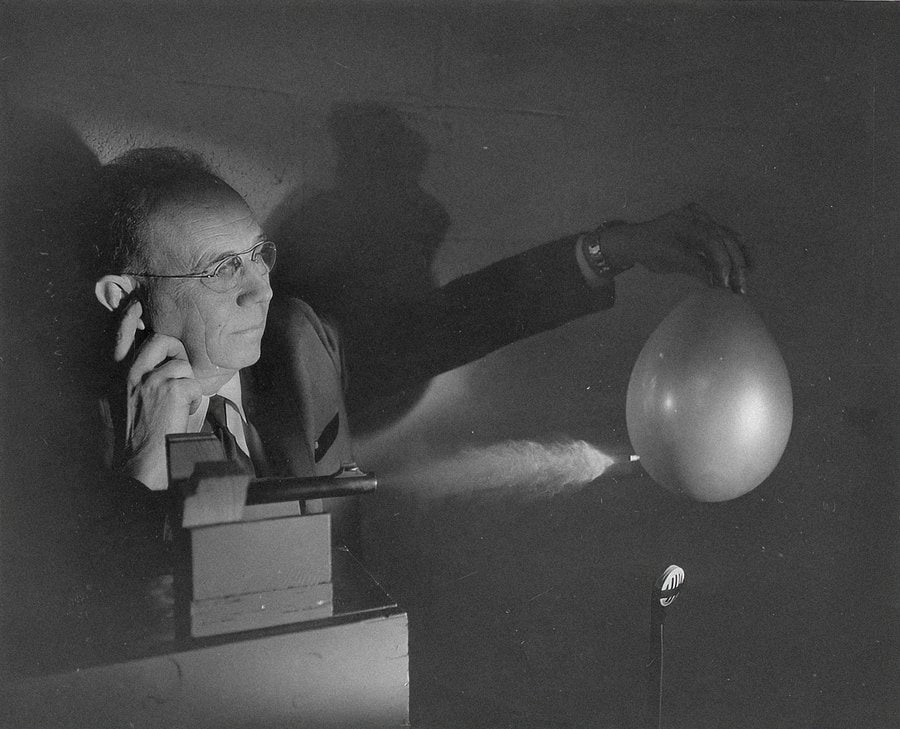
\includegraphics[width=0.45\linewidth]{1.jpg}
    \end{subfigure}
    \hfill
    \begin{subfigure}
        \centering
        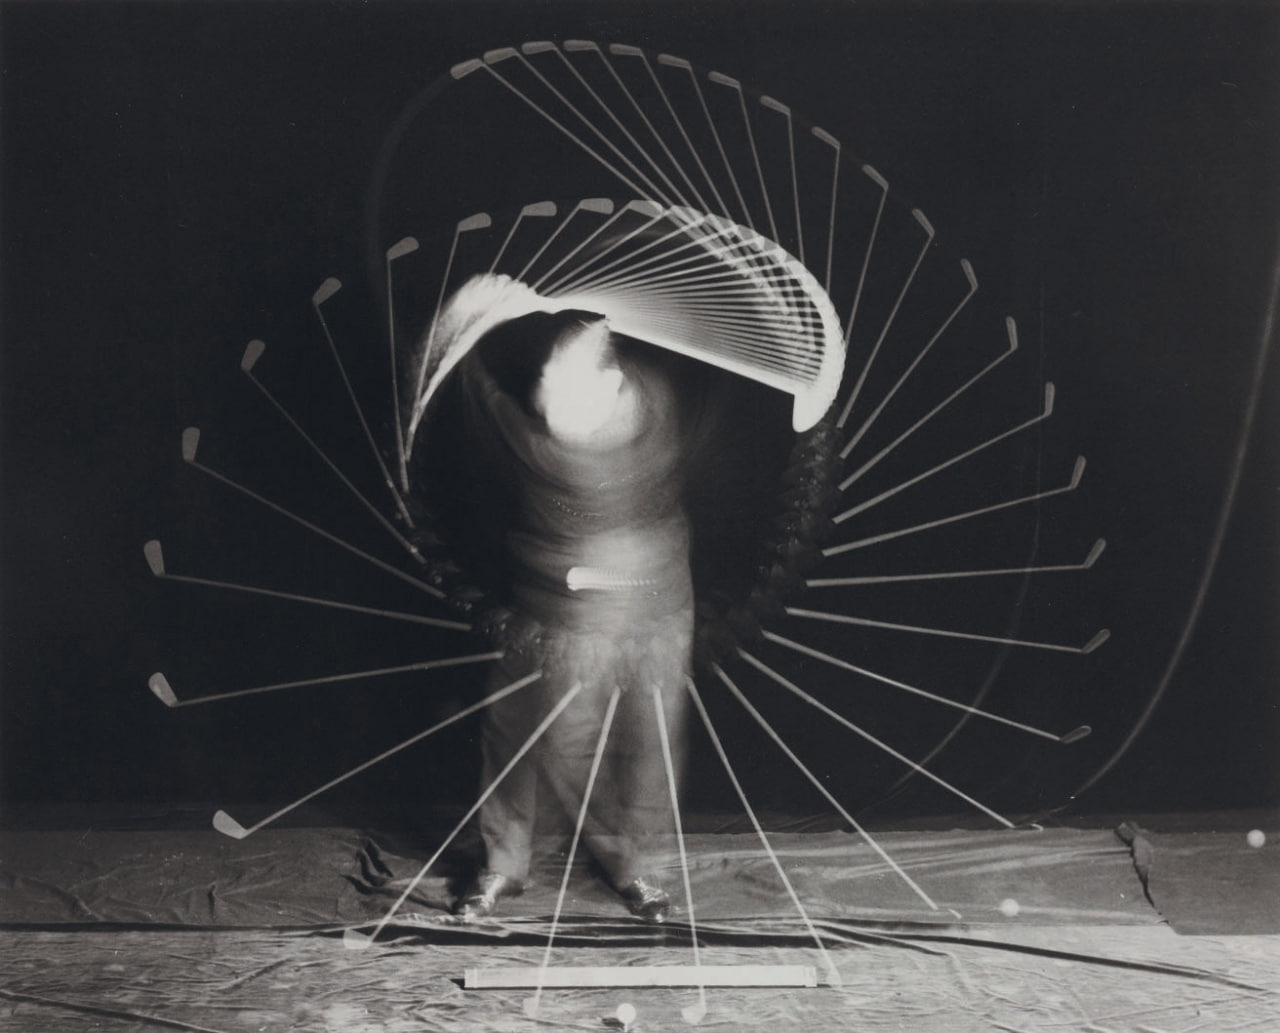
\includegraphics[width=0.45\linewidth]{2.jpg}
    \end{subfigure}
    \hfill
    \begin{subfigure}
        \centering
        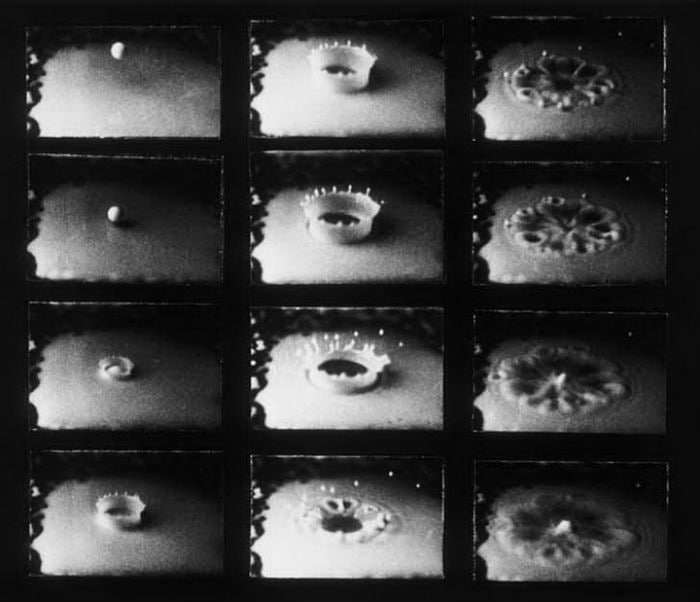
\includegraphics[width=0.45\linewidth]{4.jpg}
    \end{subfigure}
    \hfill
    \begin{subfigure}
        \centering
        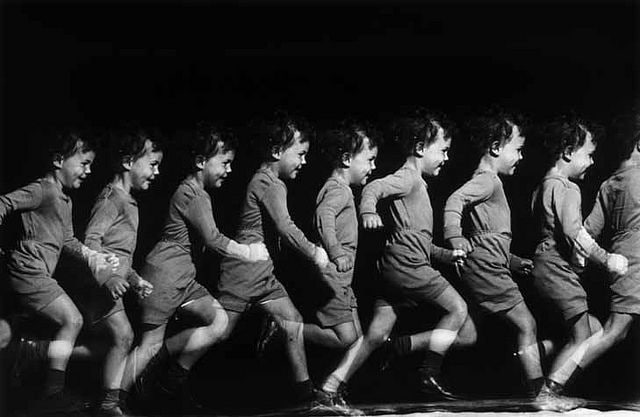
\includegraphics[width=0.45\linewidth]{6.jpg}
    \end{subfigure}
    \caption{Известные снимки Эджертона}
\end{figure}

\begin{figure}
    \centering
    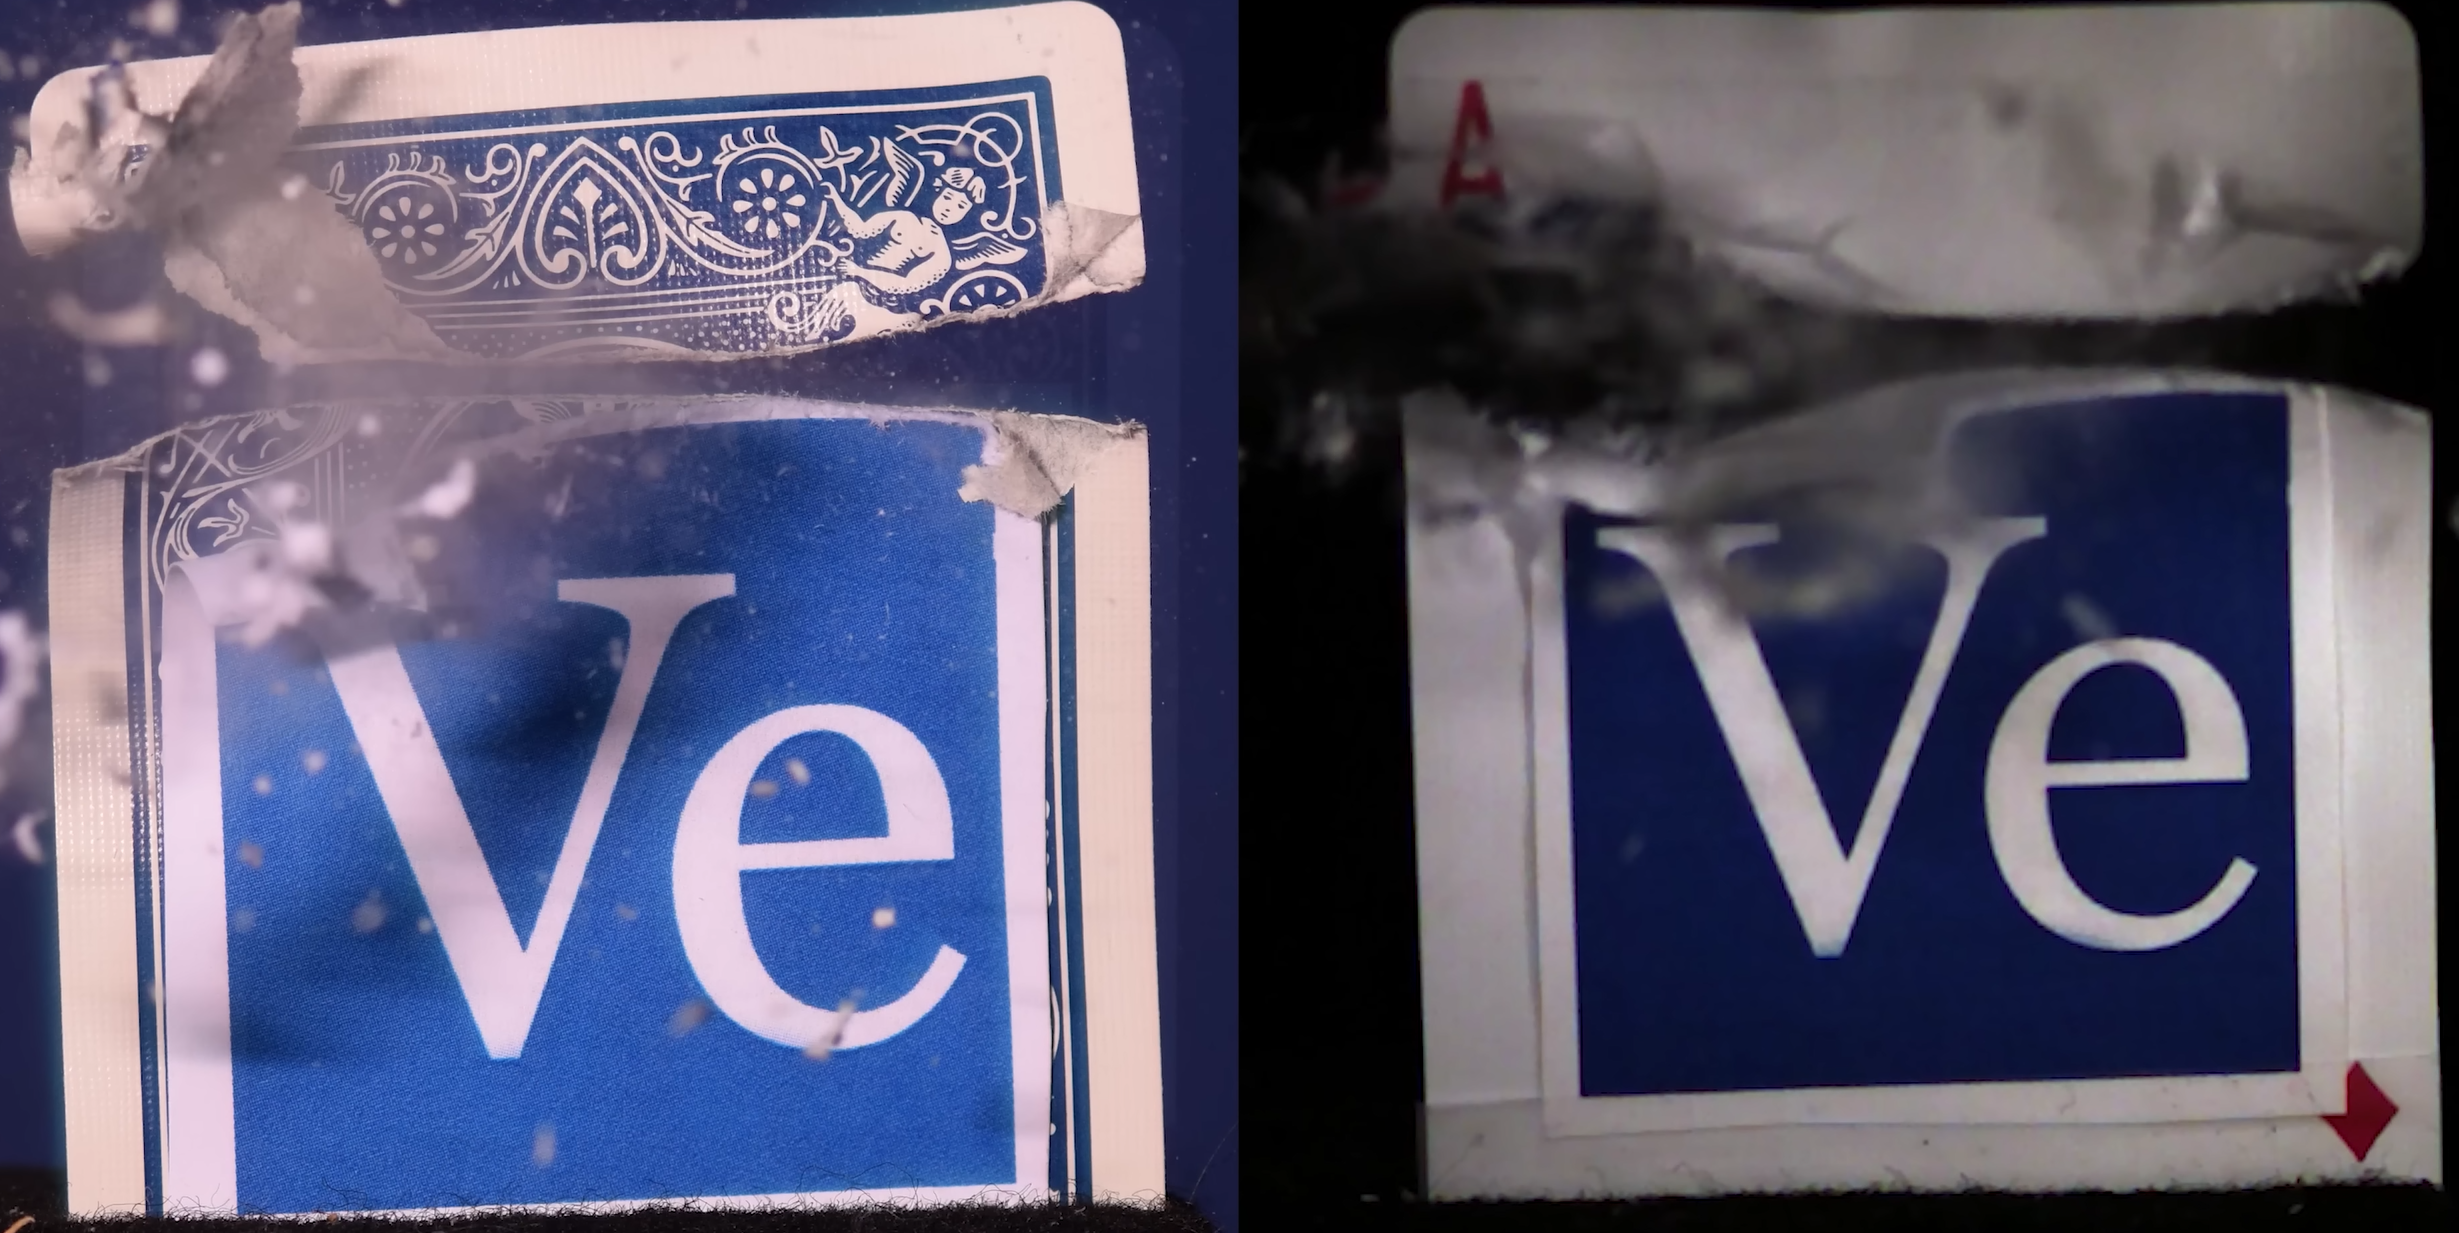
\includegraphics[width=0.5\linewidth]{13.png}
    \caption{Слева - снимок методом эджертона, справа - на высокоскоростную камеру}
    \label{fig:placeholder}
\end{figure}

Эджертон использовал звук. Микрофон улавливал резкий хлопок, будь то удар, выстрел, лопнувший шарик и через реле запускал вспышку. Для сверхзвуковых объектов (например пуль) роль сигнала играл звуковой удар, то есть ударная волна, которую создаёт пуля. Перемещая микрофон вдоль траектории можно менять момент срабатывания и тем самым выбирать в какой точке полёта снять пулю.

Снимки Эджертона широко печатались в Life и National Geographic. Позже во Второй Мировой Войне мощный стробоскоп применялся для ночной аэрофотосъёмки берегов Нормандии накануне известной высадки. Его максимальная мощность была 60 Мвт, это нужно было, чтобы осветить землю с пролетающего в нескольких километрах над ней самолета. Для понимания один запрос в гпт по словам Альтмана тратит 0,34 Вт. То есть глупые британцы вместо того чтобы сделать 176.470.588,235294117 запросов в чат гпт решили сделать одну фотографию.

\section{Пространственное и временное разрешение}

Современные высокоскоростные камеры снимают десятки тысяч кадров в секунду, но у них есть одна проблема. Это заметно на фото. Почему современная высокоскростная камера снимает в настолько плохом качестве, в то время, как каринка с помощью метода Эджертона такая четкая?

Скорость считывания пикселей с матрицы конечна (Илья сделай вид что ты удивлен). Поэтому при съёмке приходится выбирать либо много пикселей (высокое пространственное разрешение), либо много кадров (высокое временное разрешение). Например при частоте $10^6$ кадров/с размер кадра составит всего 16*128 пикселей.

Эджертон дошёл до предела в одну сторону - один кадр, но максимальное разрешение. Но есть и противоположная крайность один пиксель и частота в триллион кадров в секунду.

\section{Однопиксельная камера}

\subsection{Принцип работы}

Однопиксельная камера это детектор, способный считать отдельные фотоны. Её чувствительность настолько высока, что она реагирует буквально на каждый квант света. Камера фиксирует количество фотонов примерно триллион раз в секунду т.е один кадр соответствует интервалу в 1 пикосекунду (это секунда в -12 степени), за который свет проходит всего 0,3 мм.

Но, очевидно, один пиксель не даёт картинки. Чтобы получить изображение нужно применить алгоритм реконструкции.

\subsection{Алгоритм реконструкции}

Тут решение направшивается. Просто повтороить сцену множество раз снимая разные фрагменты. Если сцена воспроизводима, т.е каждый раз освещается одним и тем же световым импульсом, то можно снять пространство по точкам размером с 1 пиксель.

\begin{enumerate}
    \item Лазерный импульс направляется в фиксированную точку сцены.
    \item Камера направлена в конкретную точку двумя поворотными зеркалами (одно вращается по горизонтали, другое по вертикали).
    \item Запускается миллионы импульсов, все сигналы усредняются и получается один пиксель изображения.
    \item Зеркала поворачиваются, эксперимент повторяется для следующего пикселя.
    \item После прохода по всей сетке пикселей кадры объединяются в видео.
\end{enumerate}

Это такая же логика, как и у стробоскопа Эджертона. Воспроизводимость процесса позволяет замерять его по кускам и собирать полную картину. Теоретически таким способом можно получить разрешение хоть 8К, просто это займет соответственно много времени. 

\section{Квадриллион кадров в секунду}

\subsection{Зачем снимать электроны?}

Электроны создают поля, в которых происходят все химические реакции. Они запускают образование и разрушение молекулярных связей. Если бы удалось наблюдать за перераспределением электронной плотности в реальном времени, это дало бы принципиально новый инструмент для изучения материи на самом фундаментальном уровне. Так что, раузмеется, множество ученых хотят получить такой инструмент.

Для этого нужна вспышка продолжительностью в аттосекунд (10 в -15 степени). Для понимания масштаба. Отношение аттосекунды к секунде такое же, как отношение секунды к возрасту вселенной. Хах...

\subsection{Линейный ускоритель SLAC}

В Калифорнии находится линейный ускоритель электронов SLAC длиной 3,2 км, это если что самое прямое сооружение в мире. Там генерируется 120 пучков электронов в секунду, каждый разгоняется до 99,99992\percent скорости света.

Пучок проходит через ондулятор — устройство с рядами магнитов чередующейся полярности. Магнитное поле заставляет электроны колебаться. Поскольку они несут заряд, колебания генерируют электромагнитное излучение. Благодаря релятивистскому сокращению длин (электрон движется почти со скоростью света) расстояния между магнитами с точки зрения самого электрона оказываются на много порядков меньше, чем в лабораторной системе отсчёта. Это приводит к тому, что длина волны излучения сжимается до рентгеновского диапазона в около 50 пикометров. Понять это сложно (на описании съемки станет легче), да, но так работает теория относительности. Электрон настолько быстр, что расстояние для него искажается. 

Постепенно рентгеновские поля начинают группировать электроны в пучке в тонкие слои имменуемые микробанчингом. Слои излучают синхронно, и излучение становится когерентным, как лазерное. Мощность рентгеновского импульса при этом резко возрастает, а его длительность составляет единицы фемтосекунд или сотни аттосекунд. Я такие рамзмерности вообще в первый раз услышал.

\subsection{Съёмка молекулы}

Метод работает по той же логике, что и стробоскоп, и однопиксельная камера:

\begin{enumerate}
    \item Лазерный импульс попадает в молекулу и выводит её из равновесия, запуская изменение.
    \item Через заданную задержку в молекулу бьёт рентгеновский импульс. Он выбивает электрон из внутренней оболочки атома.
    \item По кинетической энергии вырванного электрона вычисляется электронная плотность вокруг атома в данный момент.
    \item Эксперимент повторяется с той же молекулой, но с увеличенной задержкой.
    \item Из серии измерений собирается видео перераспределения заряда.
\end{enumerate}

Задержку между импульсами можно менять с точностью до 300 аттосекунд, что даёт частоту съёмки порядка $10^{15}$ кадров в секунду. Ну или по русски до квадриллиона кадров в секунду. 

\section{Заключение}

Три совершенно разные технологии. Стробоскоп 1930ых, однопиксельная камера и рентгеновский лазер на ускорителе, как оказалось, работают по одному принципу: воспроизводимый процесс + короткая вспышка + повторение.

Эджертон остановил пулю одной вспышкой конденсатора. Его идея пережила его самого, прошла через ночные бомбардировщики Второй мировой и добралась до трёхкилометрового туннеля в Калифорнии, где учёные снимают то, что раньше считалось принципиально ненаблюдаемым, движение электронов внутри молекулы. 

Если вы осилили это чтиво, поздравляю вы стали умнее. Наверное)

\section*{Источники}

\begin{enumerate}[label={[\arabic*]}]
    \item Edgerton, H.\,E., Killian, J.\,R. \textit{Moments of Vision: The Stroboscopic Revolution in Photography.} MIT Press, 1979.
    \item SLAC National Accelerator Laboratory. \textit{About SLAC}. \texttt{https://www.slac.stanford.edu/about/}
    \item Duris, J. et al. \textit{Tunable isolated attosecond X-ray pulses with gigawatt peak power from a free-electron laser.} Nature Photonics, 2020.
    \item Gigan, S. et al. \textit{Roadmap on wavefront shaping and deep imaging in complex media.} Journal of Physics: Photonics, 2022. (однопиксельные методы)
\end{enumerate}

\end{document}